\documentclass[12pt,a4paper]{article}
\usepackage[utf8]{inputenc}
\usepackage{babel}
\usepackage[T1]{fontenc}
\usepackage{graphicx}
\usepackage{booktabs}
\usepackage{xcolor}
\usepackage{geometry}
\usepackage{float} 
\usepackage{hyperref}
\usepackage{verbatim} 
\usepackage{listings} % Pacote adicionado para formatar código fonte
\geometry{margin=2.5cm}
\usepackage{graphicx}
\graphicspath{{images/}}
\usepackage{float}
\usepackage{placeins}

% Configuração visual para os blocos de código Verilog
\lstset{
    language=Verilog,
    basicstyle=\ttfamily\scriptsize,
    keywordstyle=\color{blue}\bfseries,
    commentstyle=\color{gray}\itshape,
    stringstyle=\color{orange},
    breaklines=true,
    frame=single,
    numbers=left,
    numberstyle=\tiny\color{gray},
    captionpos=b,
    showstringspaces=false
}

\title{Relatorio Tecnico: Implementacao de Controlador de Cache}
\author{Arthur Carvalho Rodrigues, Débora Luiza de Paula Silva, \\ Gustavo Henrique Rodrigues de Castro e Mariana Almeida Mendonça}
\date{\today}

\begin{document}

\maketitle

\section{Introducao}
Este trabalho apresenta a implementacao e validacao de um controlador de cache em SystemVerilog, conforme os requisitos do Trabalho Pratico 1 de Arquitetura de Computadores III. O objetivo foi construir um controlador funcional entre CPU e memoria principal, com enfase em tratamento de hit/miss, politicas de leitura e escrita, substituicao de blocos e validacao por simulacao.

A arquitetura adotada foi uma cache 2-way set associative com 4 conjuntos, endereco de 8 bits, palavra de 32 bits e bloco de 1 palavra. As politicas selecionadas foram write-back, write-allocate e substituicao LRU simples por conjunto. A validacao foi feita por testbench automatizado, com cenarios de leitura, escrita, conflitos de indice, substituicao, write-back e casos limite.

\section{Implementacao}
Foi criado um módulo de topo, denominado \texttt{cache\_top}, responsável por integrar o controlador de cache e a memória principal. Esse módulo recebe os sinais da CPU, repassa as requisições ao controlador de cache e conecta internamente a interface entre o controlador e a memória principal.

Essa separação torna o projeto mais modular, pois o \texttt{cache\_controller} contém apenas a lógica de controle da cache, o \texttt{main\_memory} modela a memória principal com latência, e o \texttt{cache\_top} realiza a integração entre os dois módulos. Dessa forma, o \textit{testbench} pode validar o sistema completo a partir da interface da CPU.




\subsection{Decisoes de projeto, simplificacoes e hipoteses}
As principais decisoes tecnicas foram:
\begin{itemize}
    \item cache 2-way set associative com 4 conjuntos, por equilibrio entre simplicidade e cobertura dos cenarios exigidos;
    \item politica de escrita \textit{write-back} com bit \textit{dirty}, reduzindo trafego para memoria principal;
    \item politica de miss de escrita \textit{write-allocate}, mantendo coerencia entre caminho de leitura e escrita;
    \item substituicao LRU simples por conjunto, usando 1 bit por conjunto (suficiente para 2 vias);
    \item separacao modular em \texttt{cache\_controller}, \texttt{main\_memory} e \texttt{cache\_top}.
\end{itemize}

Simplificacoes adotadas:
\begin{itemize}
    \item bloco de cache com 1 palavra (32 bits), sem selecao de multiplas palavras por bloco;
    \item memoria principal modelada com latencia fixa de ciclos;
    \item interface CPU simplificada para sinais de leitura/escrita e handshake por \texttt{cpu\_ready}.
\end{itemize}

Hipoteses do modelo:
\begin{itemize}
    \item enderecamento por byte, com divisao do endereco em \texttt{tag[7:4]}, \texttt{index[3:2]} e \texttt{offset[1:0]};
    \item operacoes serializadas no testbench (uma requisicao por vez);
    \item coerencia externa entre CPU e memoria principal tratada apenas pelo controlador modelado.
\end{itemize}
\section{Depuração de erro temporal entre cache e memória principal}

Durante a etapa de validação funcional do controlador de cache, foram inicialmente executados testes básicos de leitura e escrita. Esses testes verificaram corretamente os seguintes cenários:

\begin{itemize}
    \item leitura com miss;
    \item leitura com hit;
    \item escrita com hit;
    \item leitura após escrita;
    \item escrita com miss utilizando \textit{write-allocate};
    \item leitura após \textit{write-allocate}.
\end{itemize}

A simulação inicial apresentou resultados coerentes para esses casos. Por exemplo, uma leitura no endereço \texttt{8'h10} resultou inicialmente em miss e retornou o valor \texttt{32'h1004}. Em seguida, uma nova leitura no mesmo endereço resultou em hit, confirmando que o bloco havia sido carregado corretamente para a cache. Também foi validado que uma escrita com hit atualizava o valor armazenado na cache e que leituras posteriores retornavam o valor atualizado.

\subsection{Identificação do problema}

Após a validação dos casos básicos, foram adicionados testes envolvendo conflitos de índice, substituição de blocos e escrita de volta para a memória principal. Esses testes utilizam endereços diferentes que mapeiam para o mesmo conjunto da cache, permitindo avaliar o comportamento da política de substituição LRU e da política de escrita \textit{write-back}.

A divisão de endereço adotada no projeto foi:

\begin{itemize}
    \item \texttt{addr[7:4]}: campo de tag;
    \item \texttt{addr[3:2]}: campo de índice;
    \item \texttt{addr[1:0]}: campo de offset.
\end{itemize}

Dessa forma, os endereços \texttt{8'h08}, \texttt{8'h18} e \texttt{8'h28} possuem o mesmo campo de índice e, portanto, mapeiam para o mesmo conjunto da cache.

Como a memória principal foi inicializada com a regra:

\begin{verbatim}
memory_array[i] = 32'h1000 + i;
\end{verbatim}

os valores esperados para esses endereços eram:

\begin{table}[h]
\centering
\begin{tabular}{|c|c|c|}
\hline
\textbf{Endereço} & \textbf{Palavra acessada} & \textbf{Valor esperado} \\
\hline
\texttt{8'h08} & 2  & \texttt{32'h1002} \\
\texttt{8'h18} & 6  & \texttt{32'h1006} \\
\texttt{8'h28} & 10 & \texttt{32'h100A} \\
\hline
\end{tabular}
\caption{Valores esperados para acessos que mapeiam para o mesmo conjunto da cache.}
\end{table}

No entanto, durante a simulação, foi observado o seguinte comportamento:

\begin{verbatim}
READ | Addr: 8'h08 | Data: 32'h1002 | Hit: 0
READ | Addr: 8'h18 | Data: 32'h1002 | Hit: 0
\end{verbatim}

O primeiro acesso estava correto, pois o endereço \texttt{8'h08} corresponde à palavra 2 da memória. Entretanto, o segundo acesso estava incorreto, pois o endereço \texttt{8'h18} deveria retornar \texttt{32'h1006}, mas retornou novamente \texttt{32'h1002}. Isso indicou que o controlador estava armazenando ou retornando um valor antigo de \texttt{mem\_rdata}.

\subsection{Causa do erro}

A causa do problema estava relacionada ao sincronismo entre os sinais \texttt{mem\_ready} e \texttt{mem\_rdata}. A memória principal foi modelada com latência, de modo que, ao final de uma operação de leitura, ela atualiza o dado de saída e sinaliza que a operação foi concluída.

A lógica da memória principal utiliza atribuições não bloqueantes:

\begin{verbatim}
mem_rdata <= memory_array[saved_word_index];
mem_ready <= 1'b1;
\end{verbatim}

Em SystemVerilog, dentro de blocos sequenciais, atribuições não bloqueantes não atualizam imediatamente os sinais. Os novos valores só ficam disponíveis após a borda de clock atual.

Na versão inicial do controlador, a cache era atualizada no mesmo ciclo em que o sinal \texttt{mem\_ready} era detectado:

\begin{verbatim}
if (mem_ready) begin
    data[req_index][victim_way] <= mem_rdata;
    cpu_rdata <= mem_rdata;
end
\end{verbatim}

Com isso, o controlador lia o valor anterior de \texttt{mem\_rdata}, e não o valor recém-produzido pela memória principal. Esse erro se tornou evidente nos testes com misses consecutivos, nos quais o dado retornado por um acesso correspondia ao acesso anterior.

\subsection{Correção adotada}

Para corrigir o problema, foi adicionado um estado intermediário à máquina de estados do controlador de cache. O fluxo anterior era:

\begin{verbatim}
ALLOCATE -> RESPOND
\end{verbatim}

Após a correção, o fluxo passou a ser:

\begin{verbatim}
ALLOCATE -> UPDATE_CACHE -> RESPOND
\end{verbatim}

O estado \texttt{ALLOCATE} passou a ser responsável apenas por solicitar a leitura da memória principal e aguardar o sinal \texttt{mem\_ready}. Quando \texttt{mem\_ready} é ativado, a máquina de estados avança para o estado \texttt{UPDATE\_CACHE}. Nesse estado, o valor de \texttt{mem\_rdata} já está estável e pode ser corretamente armazenado na cache.

O comportamento corrigido pode ser resumido da seguinte forma:

\begin{enumerate}
    \item No estado \texttt{ALLOCATE}, o controlador solicita a leitura da memória principal.
    \item A memória principal, após sua latência interna, ativa \texttt{mem\_ready}.
    \item O controlador avança para o estado \texttt{UPDATE\_CACHE}.
    \item No estado \texttt{UPDATE\_CACHE}, o dado presente em \texttt{mem\_rdata} é gravado na cache.
    \item A tag, o bit \texttt{valid}, o bit \texttt{dirty} e a informação de LRU são atualizados.
    \item No estado \texttt{RESPOND}, o controlador sinaliza \texttt{cpu\_ready}.
\end{enumerate}

Essa modificação garante que a cache não seja atualizada com dados atrasados da memória principal.

\subsection{Importância da correção}

Esse erro reforçou a importância de considerar o comportamento temporal dos sinais em projetos de hardware. Diferentemente de um programa sequencial em software, em uma descrição de hardware os sinais atualizados em blocos sequenciais não assumem seus novos valores instantaneamente.

Portanto, mesmo que o sinal \texttt{mem\_ready} indique que a memória terminou uma operação, o controlador precisa garantir que o valor de \texttt{mem\_rdata} esteja estável antes de armazená-lo na cache.

A inclusão do estado \texttt{UPDATE\_CACHE} tornou a máquina de estados mais robusta e mais coerente com o funcionamento síncrono dos módulos do projeto. Além disso, a falha foi identificada somente após a criação de testes mais completos, o que evidencia a importância de validar não apenas os casos básicos de hit e miss, mas também os cenários de conflito de índice, substituição de blocos e escrita de volta para a memória principal.

\section{Resultados e Validação Funcional}

Após a implementação do controlador de cache, foram realizados testes funcionais por meio de um \textit{testbench} em SystemVerilog. O objetivo desses testes foi validar o comportamento da cache em operações de leitura, escrita, tratamento de misses, política de substituição LRU, política \textit{write-back} e política \textit{write-allocate}.

A simulação foi executada utilizando o Icarus Verilog. O arquivo \texttt{wave.vcd} também foi gerado para permitir a visualização das formas de onda no GTKWave.

\subsection{Testes realizados}

A Tabela~\ref{tab:testes-cache} resume os principais testes realizados e os respectivos resultados obtidos.

\begin{table}[h]
\centering
\begin{tabular}{|c|p{7cm}|c|}
\hline
\textbf{Teste} & \textbf{Cenário validado} & \textbf{Resultado} \\
\hline
0 & Cache vazia apos reset (primeiro acesso deve resultar em miss) & Passou \\
\hline
0.1 & Acesso ao endereco extremo baixo (\texttt{8'h00}) & Passou \\
\hline
0.2 & Acesso ao endereco extremo alto (\texttt{8'hFF}) & Passou \\
\hline
1 & Leitura com miss e alocação do bloco na cache & Passou \\
\hline
2 & Leitura com hit após o bloco já estar na cache & Passou \\
\hline
3 & Escrita com hit utilizando política \textit{write-back} & Passou \\
\hline
4 & Leitura após escrita, confirmando atualização do dado na cache & Passou \\
\hline
5 & Escrita com miss utilizando política \textit{write-allocate} & Passou \\
\hline
6 & Leitura após \textit{write-allocate}, confirmando que o bloco foi carregado na cache & Passou \\
\hline
7 & Conflito de índice entre endereços que mapeiam para o mesmo conjunto & Passou \\
\hline
8 & Atualização da informação de LRU após novo acesso a uma via & Passou \\
\hline
9 & Substituição de bloco seguindo a política LRU & Passou \\
\hline
10 & Confirmação da substituição LRU por meio de novos acessos & Passou \\
\hline
11 & Escrita de volta de bloco marcado como \textit{dirty} & Passou \\
\hline
12 & Verificação de que a memória principal foi atualizada após o \textit{write-back} & Passou \\
\hline
\end{tabular}
\caption{Resumo dos testes funcionais realizados no controlador de cache.}
\label{tab:testes-cache}
\end{table}

\subsection{Validação de leitura com miss e hit}

Inicialmente, foi realizada uma leitura no endereço \texttt{8'h10}. Como a cache estava vazia após o reset, o acesso resultou em miss. O controlador buscou o dado correspondente na memória principal, carregou o bloco na cache e retornou o valor \texttt{32'h1004}.

Em seguida, uma nova leitura para o mesmo endereço foi realizada. Dessa vez, o dado já estava presente na cache, resultando em hit.

\begin{verbatim}
READ  | Addr: 8'h10 | Data: 32'h1004 | Hit: 0
READ  | Addr: 8'h10 | Data: 32'h1004 | Hit: 1
\end{verbatim}

Esse resultado confirma o funcionamento correto do caminho de leitura, tanto para miss quanto para hit.

\subsection{Validação de escrita com hit e política write-back}

Após o carregamento do endereço \texttt{8'h10} na cache, foi realizada uma escrita nesse mesmo endereço com o valor \texttt{32'hdeadbeef}. Como o bloco já estava presente na cache, a operação resultou em hit. O dado foi atualizado na cache e a linha foi marcada como \textit{dirty}, conforme a política \textit{write-back}.

Uma leitura posterior no mesmo endereço retornou o valor atualizado:

\begin{verbatim}
WRITE | Addr: 8'h10 | Data: 32'hdeadbeef | Hit: 1
READ  | Addr: 8'h10 | Data: 32'hdeadbeef | Hit: 1
\end{verbatim}

Esse teste confirma que a escrita com hit atualiza corretamente a cache sem escrever imediatamente na memória principal.

\subsection{Validação de escrita com miss e política write-allocate}

Também foi testada uma escrita em um endereço ainda não presente na cache, \texttt{8'h24}, com o valor \texttt{32'hcafebabe}. Como o bloco não estava na cache, ocorreu um miss. Pela política \textit{write-allocate}, o bloco foi alocado na cache e, em seguida, o valor da escrita foi armazenado.

A leitura posterior do mesmo endereço resultou em hit e retornou o valor escrito:

\begin{verbatim}
WRITE | Addr: 8'h24 | Data: 32'hcafebabe | Hit: 0
READ  | Addr: 8'h24 | Data: 32'hcafebabe | Hit: 1
\end{verbatim}

Esse resultado confirma que a política \textit{write-allocate} foi implementada corretamente.

\subsection{Validação de conflitos de índice e substituição LRU}

Para validar a política de substituição, foram utilizados endereços que mapeiam para o mesmo conjunto da cache. Considerando a divisão de endereço adotada:

\begin{itemize}
    \item \texttt{addr[7:4]}: tag;
    \item \texttt{addr[3:2]}: índice;
    \item \texttt{addr[1:0]}: offset.
\end{itemize}

Os endereços \texttt{8'h08}, \texttt{8'h18} e \texttt{8'h28} possuem o mesmo campo de índice e, portanto, mapeiam para o mesmo conjunto.

Primeiro, os endereços \texttt{8'h08} e \texttt{8'h18} foram acessados, preenchendo as duas vias do conjunto. Em seguida, o endereço \texttt{8'h08} foi acessado novamente, atualizando a informação de LRU e tornando \texttt{8'h18} o bloco menos recentemente usado. Ao acessar \texttt{8'h28}, ocorreu um miss e o controlador substituiu o bloco correspondente a \texttt{8'h18}.

A sequência observada foi:

\begin{verbatim}
READ | Addr: 8'h08 | Data: 32'h1002 | Hit: 0
READ | Addr: 8'h18 | Data: 32'h1006 | Hit: 0
READ | Addr: 8'h08 | Data: 32'h1002 | Hit: 1
READ | Addr: 8'h28 | Data: 32'h100a | Hit: 0
READ | Addr: 8'h08 | Data: 32'h1002 | Hit: 1
READ | Addr: 8'h18 | Data: 32'h1006 | Hit: 0
\end{verbatim}

O último acesso a \texttt{8'h18} resultou em miss, confirmando que esse foi o bloco substituído. Isso valida o funcionamento da política LRU simples adotada no projeto.

\subsection{Validação de write-back com bloco dirty}

Por fim, foi validado o comportamento de escrita de volta para a memória principal. Para isso, foi realizada uma escrita no endereço \texttt{8'h0C} com o valor \texttt{32'h11111111}. Como o endereço não estava na cache, ocorreu um miss, seguido de alocação do bloco e atualização da linha, que passou a ser marcada como \textit{dirty}.

Em seguida, foram realizados acessos a outros endereços que mapeiam para o mesmo conjunto, forçando a substituição do bloco correspondente a \texttt{8'h0C}. Como esse bloco estava marcado como \textit{dirty}, o controlador precisou escrever seu conteúdo de volta na memória principal antes de substituí-lo.

A sequência relevante foi:

\begin{verbatim}
WRITE | Addr: 8'h0c | Data: 32'h11111111 | Hit: 0
READ  | Addr: 8'h1c | Data: 32'h1007     | Hit: 0
READ  | Addr: 8'h1c | Data: 32'h1007     | Hit: 1
READ  | Addr: 8'h2c | Data: 32'h100b     | Hit: 0
READ  | Addr: 8'h0c | Data: 32'h11111111 | Hit: 0
\end{verbatim}

O último acesso ao endereço \texttt{8'h0C} resultou em miss, pois o bloco havia sido substituído. Entretanto, o valor retornado foi \texttt{32'h11111111}, confirmando que o dado modificado foi corretamente escrito de volta na memória principal durante o processo de substituição.

Esse teste valida o funcionamento conjunto da política \textit{write-back}, do bit \textit{dirty} e da substituição de blocos.

\subsection{Casos limite: cache vazia e enderecos extremos}
Foram adicionados testes explicitos para os casos limite exigidos no enunciado:
\begin{itemize}
    \item cache vazia apos reset: primeiro acesso ao endereco \texttt{8\'h10} deve resultar em miss;
    \item acesso ao endereco extremo baixo \texttt{8\'h00};
    \item acesso ao endereco extremo alto \texttt{8\'hFF}.
\end{itemize}

Trecho representativo do log de simulacao:
\begin{verbatim}
--- TESTE 0: Cache vazia apos reset (primeiro acesso deve ser miss) ---
READ  | Addr: 8\'h10 | Data: 32\'h1004 | Hit: 0
--- TESTE 0.1: Endereco extremo baixo (8\'h00) ---
READ  | Addr: 8\'h0  | Data: 32\'h1000 | Hit: 0
--- TESTE 0.2: Endereco extremo alto (8\'hFF) ---
READ  | Addr: 8\'hff | Data: 32\'h103f | Hit: 0
\end{verbatim}

Esses resultados confirmam o comportamento esperado para inicializacao da cache e para limites do espaco de enderecamento.
\subsection{Conclusão da validação}

Os testes realizados cobriram os principais comportamentos esperados do controlador de cache: leitura com hit e miss, escrita com hit e miss, alocação em miss de escrita, substituição por LRU, conflitos de índice e escrita de volta de blocos modificados. Todos os testes apresentaram os resultados esperados, indicando que o controlador implementado atende à especificação definida para o projeto.


\begin{figure}[H]
\centering
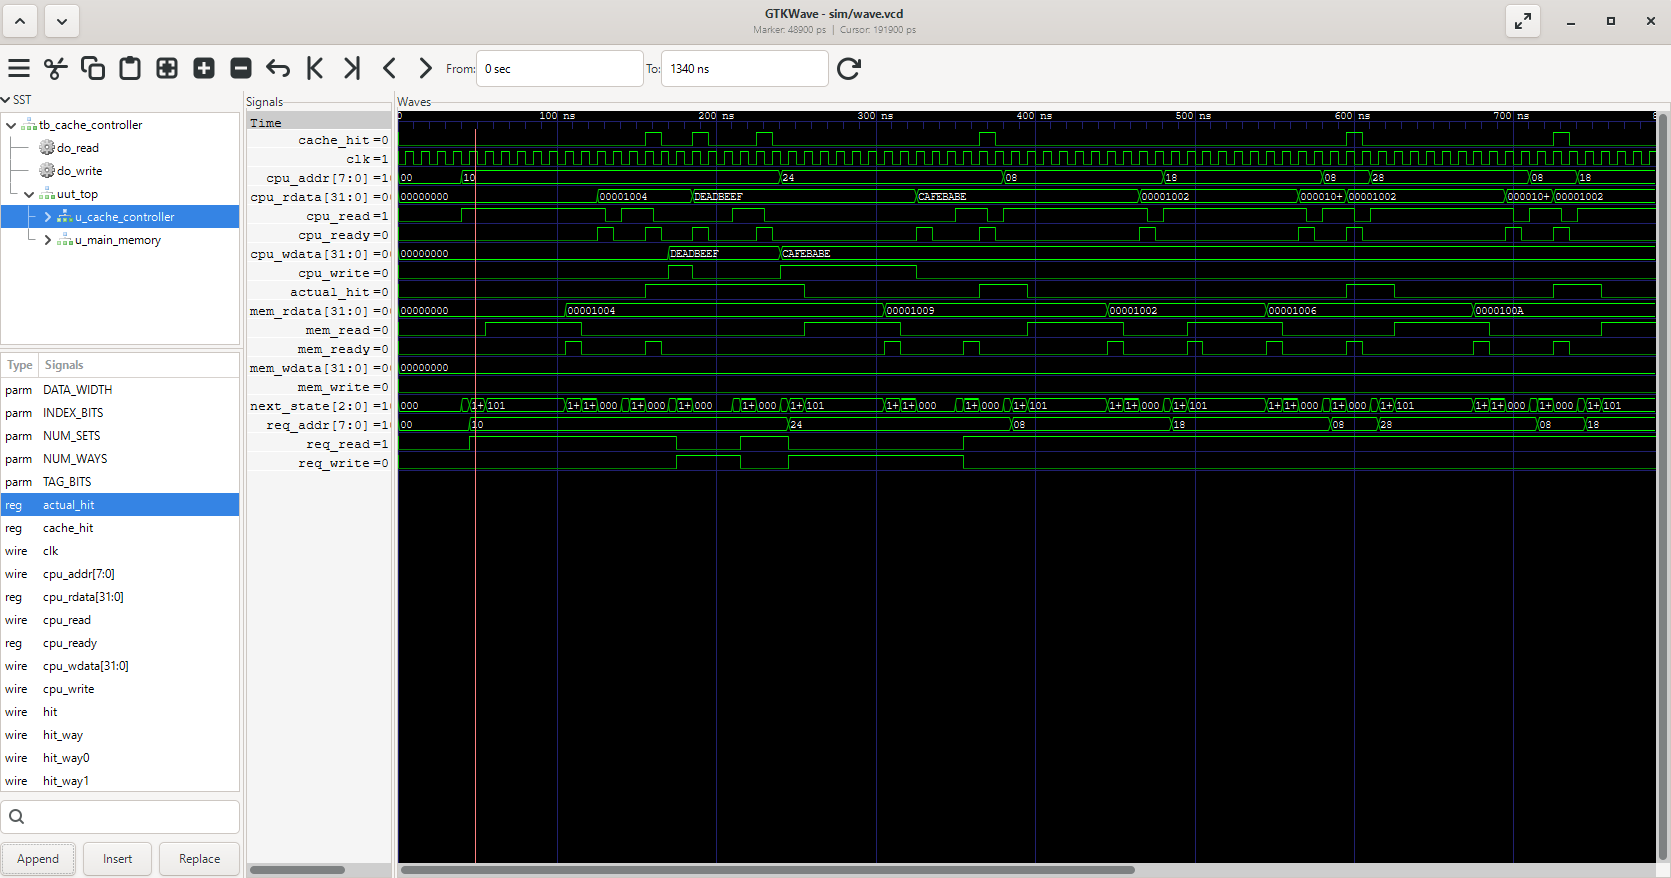
\includegraphics[width=\textwidth]{visaoGeral.png}
\caption{Visão geral da simulação do controlador de cache, mostrando operações de leitura, escrita, misses, hits, substituição LRU e write-back.}
\label{fig:waveform-geral}
\end{figure}
\FloatBarrier

A Figura~\ref{fig:waveform-geral} apresenta uma visão geral da simulação. É possível observar a sequência de acessos realizados pelo testbench, com variação dos sinais \texttt{cpu\_addr}, \texttt{cpu\_rdata}, \texttt{cache\_hit}, \texttt{mem\_read}, \texttt{mem\_write} e \texttt{cpu\_ready}. Os pulsos de \texttt{mem\_read} ocorrem nos acessos com miss, enquanto os pulsos de \texttt{mem\_write} aparecem durante a escrita de volta de um bloco marcado como \textit{dirty}.


\begin{figure}[H]
\centering
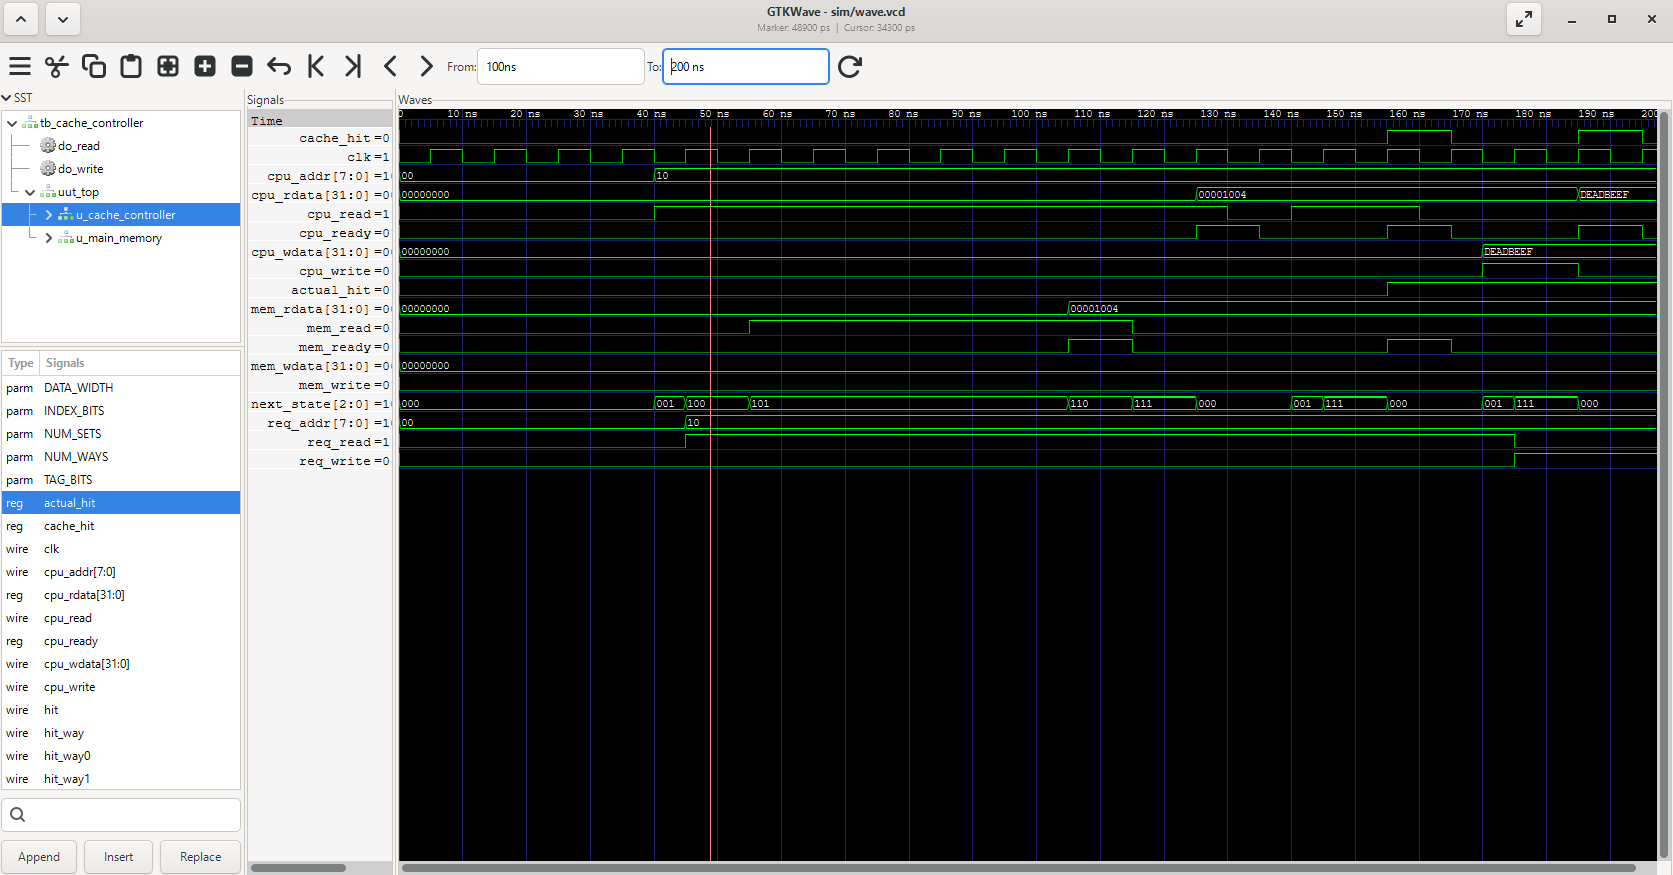
\includegraphics[width=\textwidth]{readMisseHit.png}
\caption{Validação de leitura com miss seguida de leitura com hit para o endereço \texttt{8'h10}. No primeiro acesso, o controlador ativa \texttt{mem\_read} e retorna o dado \texttt{32'h1004}. No segundo acesso ao mesmo endereço, o sinal \texttt{cache\_hit} é ativado, indicando que o dado já estava presente na cache.}
\label{fig:waveform-read-miss-hit}
\end{figure}
\FloatBarrier

A Figura~\ref{fig:waveform-read-miss-hit} mostra a validação do caminho de leitura. Inicialmente, a CPU solicita uma leitura no endereço \texttt{8'h10}. Como a cache estava vazia após o reset, o acesso resulta em miss, indicado por \texttt{cache\_hit = 0}. O controlador então ativa \texttt{mem\_read}, aguarda o sinal \texttt{mem\_ready} da memória principal e retorna o dado \texttt{32'h1004} para a CPU.

Em seguida, o mesmo endereço é acessado novamente. Dessa vez, o bloco já está presente na cache, e o sinal \texttt{cache\_hit} é ativado. O dado é retornado diretamente pela cache, validando o funcionamento correto de uma leitura com hit.

\begin{figure}[H]
\centering
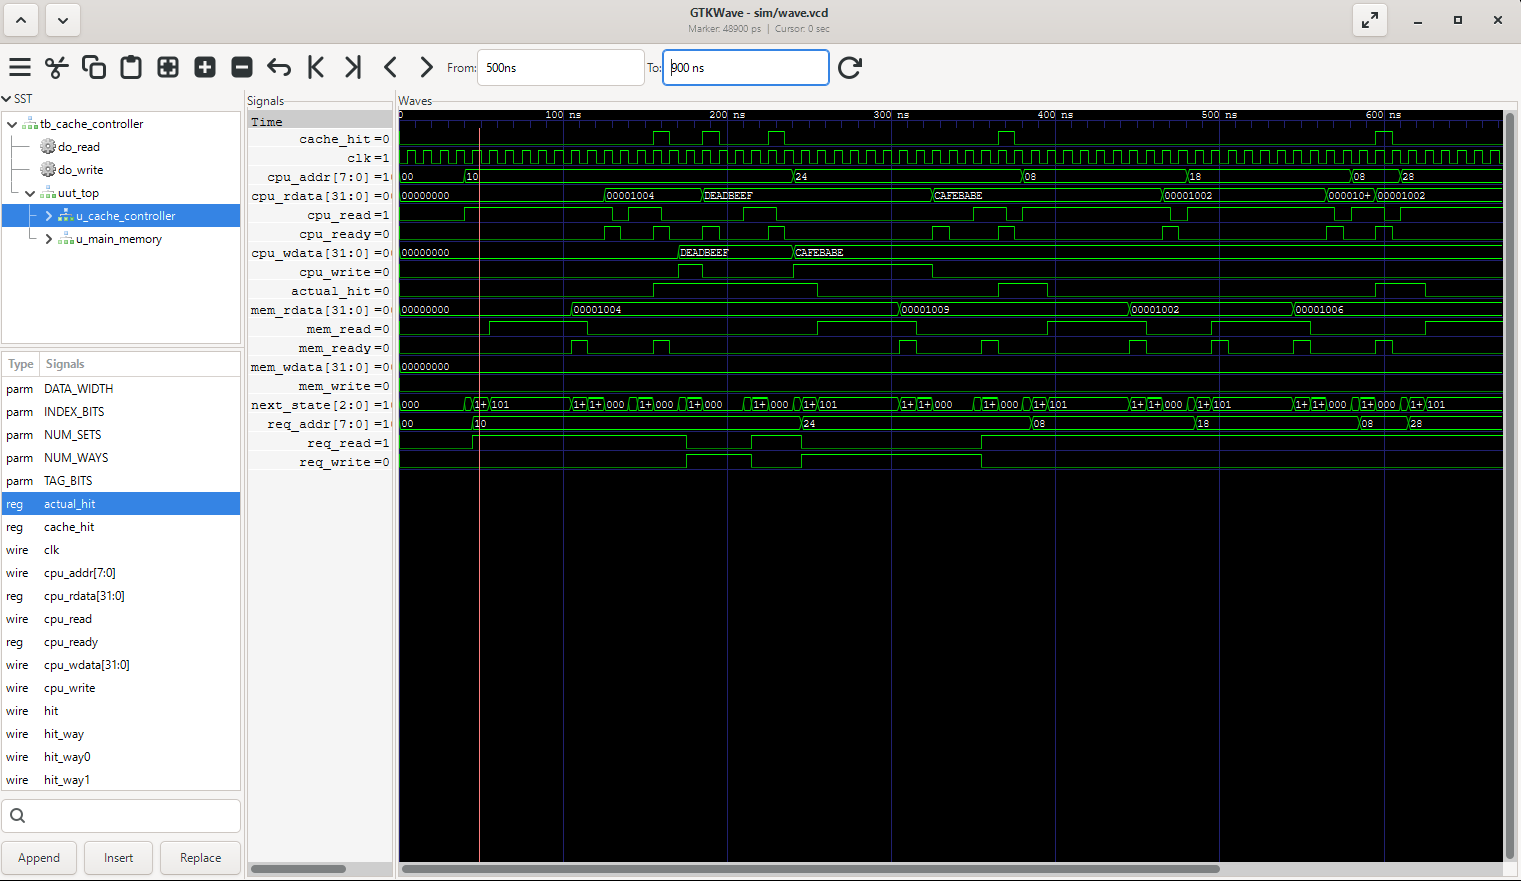
\includegraphics[width=\textwidth]{lru.png}
\caption{Validação da política de substituição LRU. Os endereços \texttt{8'h08}, \texttt{8'h18} e \texttt{8'h28} mapeiam para o mesmo conjunto da cache. Após o novo acesso a \texttt{8'h08}, esse bloco se torna o mais recentemente usado. Assim, quando \texttt{8'h28} é carregado, o bloco correspondente a \texttt{8'h18} é substituído.}
\label{fig:waveform-lru}
\end{figure}
\FloatBarrier

Na Figura~\ref{fig:waveform-lru}, observa-se a sequência de acessos utilizada para validar a política LRU. Primeiro, os endereços \texttt{8'h08} e \texttt{8'h18} são carregados no mesmo conjunto da cache. Em seguida, o endereço \texttt{8'h08} é acessado novamente, atualizando a informação de LRU. Quando o endereço \texttt{8'h28}, que também mapeia para o mesmo conjunto, é acessado, o controlador substitui o bloco menos recentemente usado, correspondente a \texttt{8'h18}. Isso é confirmado pelo fato de que uma leitura posterior de \texttt{8'h08} resulta em hit, enquanto uma leitura de \texttt{8'h18} resulta em miss.


\begin{figure}[H]
    \centering
    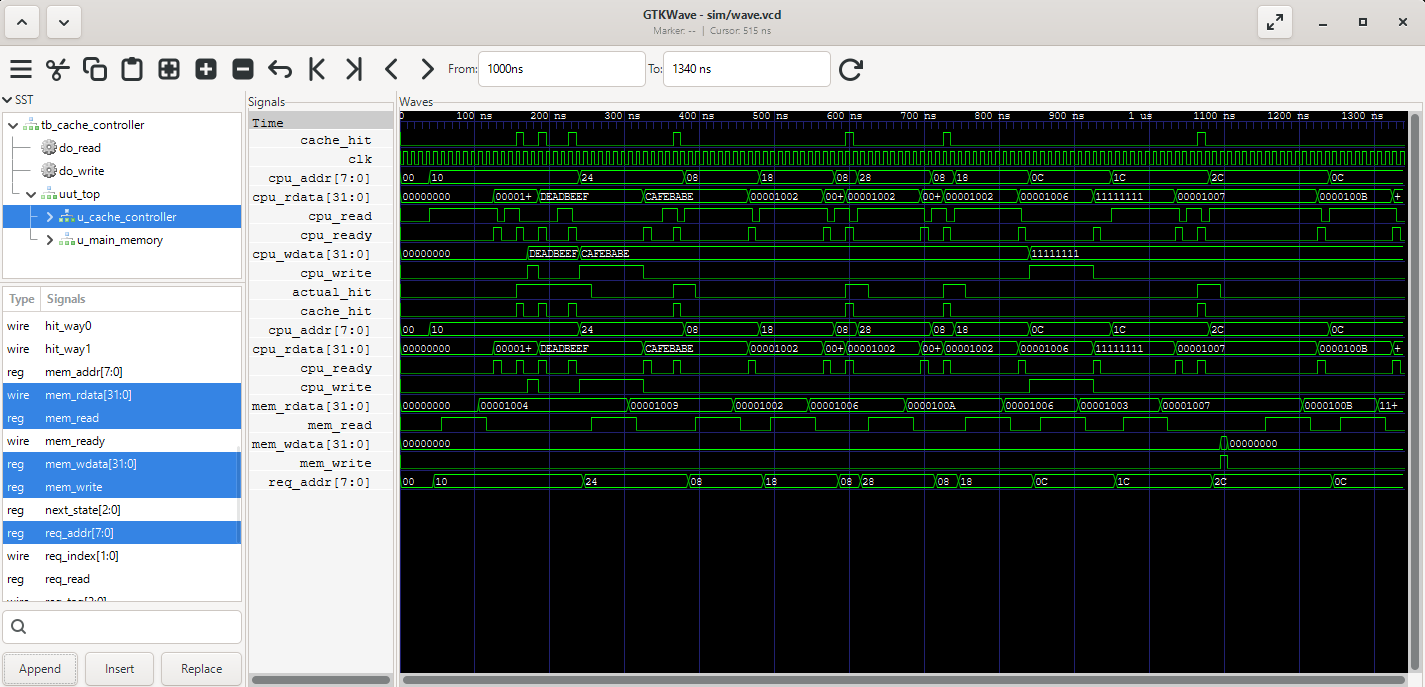
\includegraphics[width=\textwidth]{final.png}
    \caption{Validação da política \textit{write-back}. A forma de onda mostra a sequência de acessos envolvendo os endereços \texttt{8'h0C}, \texttt{8'h1C} e \texttt{8'h2C}. Após a escrita do valor \texttt{32'h11111111} no endereço \texttt{8'h0C}, o bloco é marcado como \textit{dirty}. Posteriormente, ao ocorrer a substituição desse bloco, o controlador ativa o sinal \texttt{mem\_write}, escrevendo o valor atualizado de volta na memória principal.}
    \label{fig:waveform-writeback}
\end{figure}
\FloatBarrier

A Figura~\ref{fig:waveform-writeback} apresenta a validação da política \textit{write-back}. Inicialmente, ocorre uma escrita no endereço \texttt{8'h0C} com o valor \texttt{32'h11111111}. Como a política adotada é \textit{write-back}, esse valor é atualizado na cache e a linha correspondente é marcada como \textit{dirty}, sem escrita imediata na memória principal.

Em seguida, são realizados acessos aos endereços \texttt{8'h1C} e \texttt{8'h2C}, que mapeiam para o mesmo conjunto da cache. Esses acessos forçam a substituição do bloco associado ao endereço \texttt{8'h0C}. Como esse bloco estava marcado como \textit{dirty}, o controlador ativa o sinal \texttt{mem\_write}, realizando a escrita de volta para a memória principal.

A validação funcional é complementada pelo log da simulação, no qual uma leitura posterior do endereço \texttt{8'h0C} retorna o valor \texttt{32'h11111111}. Isso confirma que o dado modificado foi corretamente preservado na memória principal após a substituição do bloco.

\section{Conclusao}
O controlador de cache implementado atende aos requisitos funcionais do trabalho para leitura, escrita, tratamento de miss, substituicao LRU, write-back e write-allocate. A validacao por simulacao demonstrou comportamento coerente tanto em cenarios basicos quanto em cenarios de conflito, substituicao e escrita de volta para memoria principal.

Como resultado, o projeto entregue contem codigo-fonte em SystemVerilog, testbench automatizado, script de simulacao, log de execucao e relatorio tecnico com evidencias. A documentacao de uso de IA foi incluida com os prompts utilizados e a descricao objetiva de como a ferramenta apoiou especificacao, implementacao e depuracao.
\section{Documentação do Uso de Inteligência Artificial (Seção 8)}
\label{sec:ia_documentation}

Em conformidade com as diretrizes de transparência do trabalho, os prompts abaixo representam as interações reais realizadas com a IA durante o desenvolvimento do projeto.

\subsection{Fase 1: Estruturação e Especificação}
\textbf{Prompt 1:}
\begin{verbatim}
Envio acima meu trabalho prático de Arquitetura de Computadores III, peço que me 
explique o que exatamente um controlador de cache precisa e me ajude a estruturar 
os passos do trabalho.
[Arquivo anexado: Trabalho Prático 1.pdf]
\end{verbatim}

\textbf{Prompt 2:}
\begin{verbatim}
Nós faremos com as seguintes especificações:
Cache 2-way set associative, N conjuntos, Política write-back, Política 
write-allocate, Substituição LRU.
Endereço: 8 bits, Tamanho da palavra: 32 bits, Número de conjuntos: 4, 
Associatividade: 2-way, Total de linhas: 8 linhas, Tamanho do bloco: 1 palavra.
\end{verbatim}

\subsection{Fase 2: Desenvolvimento do Controlador (cache\_controller.sv)}
\textbf{Prompt 3:}
\begin{verbatim}
perfeito, podemos seguir para a geração em verilog. a ordem de pastas será a que 
enviei em anexo, gostaria de começar pela cache_controller.sv
já comecei definindo os parâmetros com as informações que te enviei acima
[Trecho de código enviado]
me ajude com o restante do arquivo a partir disso
\end{verbatim}

\textbf{Prompt 4 (Refinamento de Lógica):}
\begin{verbatim}
Seguinte, não entendi alguns pontos.
não entendi por que você colocou o offset com 2 bits.
outro problema no miss, ele sempre usa lru_way, mesmo se houver uma via inválida 
livre. Também falta atualizar o LRU depois de carregar um bloco da memória.
\end{verbatim}

\subsection{Fase 3: Desenvolvimento da Memória (main\_memory.sv)}
\textbf{Prompt 5:}
\begin{verbatim}
assim ficou com algumas modificações que fiz [Arquivo cache_controller.sv anexado].
fiz as modificações indicadas, o que acha? 
após a aprovação gostaria de iniciar o desenvolvimento da memória principal.
Como o nosso barramento de endereço tem 8 bits, o espaço total de endereçamento é 
de 2^8 = 256 bytes, correto?
\end{verbatim}

\textbf{Prompt 6 (Ajuste de Latência):}
\begin{verbatim}
como a operação pode demorar um ciclo a mais do que o esperado ao invés de 
delay_counter <= LATENCY ; coloquei como delay_counter <= LATENCY - 1;
além de que a memória não guarda a operação internamente, modifiquei isso também, 
retirei alguns comentários [Arquivo main_memory.sv anexado]
\end{verbatim}

\subsection{Fase 4: Validação e Testes (tb\_cache\_controller.sv)}
\textbf{Prompt 7:}
\begin{verbatim}
gostaria de já começarmos as simulações de leitura e escrita
\end{verbatim}

\textbf{Prompt 8:}
\begin{verbatim}
como rodar esses testes pelo terminal? estou no windows
\end{verbatim}

\textbf{Prompt 9:}
\begin{verbatim}
perfeito, criei um arquivo run.sh e rodando ele obtive os resultados:
[Log do terminal enviado provando o funcionamento]
\end{verbatim}

\textbf{Prompt 10:}
\begin{verbatim}
seria algo dessa forma? fiz todos os testes necessários no arquivo em anexo, 
valide por favor [Arquivo tb_cache_controller.sv anexado com os testes de limite]
\end{verbatim}
\end{document}







